\documentclass[a4paper]{sbgames}               % final
%\usepackage[scaled=.92]{helvet}
\usepackage{times}
\usepackage{graphicx}

%% use this for zero \parindent and non-zero \parskip, intelligently.
\usepackage{parskip}

%% the 'caption' package provides a nicer-looking replacement
\usepackage[labelfont=bf,textfont=it]{caption}

\usepackage{listings}
\usepackage{color}

\definecolor{dkgreen}{rgb}{0,0.6,0}
\definecolor{gray}{rgb}{0.5,0.5,0.5}
\definecolor{mauve}{rgb}{0.58,0,0.82}

\lstset{frame=tb,
  language=C,
  aboveskip=3mm,
  belowskip=3mm,
  showstringspaces=false,
  columns=flexible,
  basicstyle={\small\ttfamily},
  numbers=none,
  numberstyle=\tiny\color{gray},
  keywordstyle=\color{blue},
  commentstyle=\color{dkgreen},
  stringstyle=\color{mauve},
  breaklines=true,
  breakatwhitespace=true,
  tabsize=3
}

\usepackage{url}
\usepackage[utf8]{inputenc}
%% Paper title.
\title{Computer Graphics}

%% Author and Affiliation (multiple authors). Use: and between authors

\author{Alexandre Tolstenko Nogueira\\InfiniBrains\\tolstenko@infinibrains.com.br 
%        \and Name2 B. Surname2\\ Name3 C. Surname3\\ ZZZZ University
%        \and Name4 D. Surname4\\ Farwest Research Center 
}
\contactinfo{\{name1,name3\}@xxx.yyyy.yyy \\
             *name2@zzzz.vvvv.vvv
}
%% Keywords that describe your work.
\keywords{Real-time Strategy, Relief Mapping, Shortest Path Algorithm, First Person Shooting}

%% Start of the paper
% Attention: As you need to insert EPS images in Postscript, 
% you need to insert PDF images into PDFs. 
% In the text, extensions cancbe omitted (latex use .eps, pdflatex get .pdf) 
% To convert them: epstopdf myimage.eps
\begin{document}

%\teaser{
%  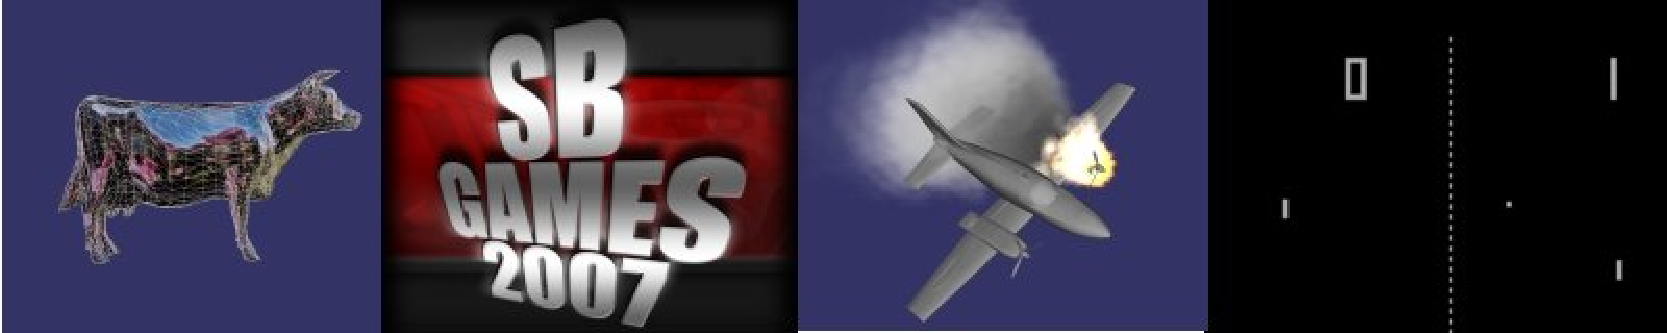
\includegraphics[width=\linewidth]{sample.pdf}
%  \caption{Optional image}
%}

%% The ``\maketitle'' command must be the first command after the
%% ``\begin{document}'' command. It prepares and prints the title block.

\maketitle

%% Abstract section.

%\begin{abstract}
%  This meta-paper describes the model to be used in papers and posters
%  for SBGames. In the subsection Author's contact, make reference to
%  the same symbol used in the affiliation.
%\end{abstract}

%% The ``\keywordlist'' command prints out the keywords.
%\keywordlist
%\contactlist

\section{Atividade Aula 3 - XXXXXXXXXXXXXX}

\subsection*{Questionário}

\textbf{1) Defina histograma e explique qual é o tipo de informação que pode ser dele retirada}

É a distribuição de frequências. É um vetor de valores onde cada um representa a somatória de quantas vezes aquele valor/intensidade apareceu no conjunto estudado. Usualmente é representado como um gráfico de colunas onde cada uma representa uma classe 

\textbf{2) Além das fórmulas de distâncias citadas, procure na literatura mais uma fórmula e explique a diferença dela para a Distância Euclidiana. Dica: procurar nas bibliotecas digitais indicadas na aula anterior. Cite as referências bibliográficas
utilizadas.
}

\textbf{3) Construa um programa para implementar e mostrar o histograma de uma imagem qualquer. O algoritmo deve receber como parâmetro uma matriz que armazena o conjunto de pixels da imagem. Além do código fonte, deverão ser entregues pelo menos dois exemplos de processamento. Não podem ser usados métodos/funções prontos de bibliotecas para construir o histograma.}

\textbf{4) Implemente um programa (método, procedimento, função) em qualquer
linguagem de programação que receba uma imagem e a exiba com todos
os pixels mais claros ou mais escuros. O nível de clareamento ou
escurecimento, assim como a matriz de pixels, devem ser recebidos
como parâmetros. Além do código fonte, deverão ser entregues dois
exemplos de processamento. Não podem ser usados métodos/funções
prontos provenientes de bibliotecas.}

\textbf{5) Continuar a implementação do programa iniciado no Exercício 4, incluindo UMA das seguintes funcionalidades:}

\begin{itemize}
\item filtro de média
\item filtro de mediana
\item equalização
\item filtro passa-alta
\end{itemize}

\textbf{6)  Para cada uma das funcionalidades dos exercícios anteriores (4 e 5):}
\begin{itemize}
\item processar uma imagem escolhida por você e mostrar a imagem original, a imagem processada e seus respectivos histogramas;
\item escrever um parágrafo explicando o efeito do filtro implementado sobre a
imagem processada.
\end{itemize}

\textbf{7) Preparação da próxima aula:}
\begin{itemize}
\item Conceitue gradiente de uma função unidimensional e gradiente de uma função bidimensional. Para que são usados? Dê um exemplo (máximo :
uma página)
\item Faça um resumo sobre introdução à geometria projetiva, incluindo
conceitos básicos e modelo de câmera virtual (máximo: uma página)
\item Faça uma comparação entre Geometria Projetiva e Geometria Euclidiana.
Citar as referências usadas (máximo: meia página)
\end{itemize}

\begin{lstlisting}
// cada dot quadrado tem 8 bits
// como a largura nao pode ser fracionada, escolhi cortar com com a funcao floor a dimensao
// floor(dpi*altura/2.54)*floor(dpi*largura/2.54)*RC -> bits
\end{lstlisting}

\textbf{2a) altura=3cm, largura=5cm, RC = 8 bits, RE=300dpi
}\begin{lstlisting}
// floor(dpi*altura/2.54) * floor(dpi*largura/2.54) * RC
354*590*8 =
            1670880 bits
            208860 bytes
            204 KiB
\end{lstlisting}

\textbf{2b) altura=3cm, largura=5cm, RC = 16 bits, RE=300dpi}
\begin{lstlisting}
// floor(dpi*altura/2.54) * floor(dpi*largura/2.54) * RC
354*590*16 =
             3341760 bits
             417720 bytes
             408 KiB
\end{lstlisting}
\pagebreak
\textbf{2c) altura=3cm, largura=5cm, RC = 16 bits, RE=600dpi}
\begin{lstlisting}
// floor(dpi*altura/2.54) * floor(dpi*largura/2.54) * RC
708*1181*16 =
              13378368 bits
              1672298 bytes
              1633 KiB
              1.6 MiB
\end{lstlisting}

\textbf{2d) altura=6cm, largura=10cm, RC = 8 bits, RE=300dpi}
\begin{lstlisting}
// floor(dpi*altura/2.54) * floor(dpi*largura/2.54) * RC
708*1181*8 =
              6689184 bits
              836148 bytes
              817 KiB
\end{lstlisting}

\textbf{2e) altura=6cm, largura=10cm, RC = 16 bits, RE=300dpi}
\begin{lstlisting}
// floor(dpi*altura/2.54) * floor(dpi*largura/2.54) * RC
708*1181*16 =
              13378368 bits
              1672298 bytes
              1633 KiB
              1.6 MiB
\end{lstlisting}

\textbf{2f) altura=6cm, largura=10cm, RC = 16 bits, RE=600dpi}
\begin{lstlisting}
// floor(dpi*altura/2.54) * floor(dpi*largura/2.54) * RC
1417*2362*16 =
              53551264 bits
              6693908 bytes
              6537 KiB
              6.4 MiB
\end{lstlisting}

\textbf{3) Procure um artigo que faça estudos sobre a resolução de contraste e/ou resolução espacial. Apresente um resumo de no máximo 20 linhas deste artigo, focando na questão de resolução. Artigo deve estar classificado no sistema Qualis (área de Ciência da Computação) (ver dicas adiante) Principais sites para busca de artigos científicos:}
\begin{itemize}
\item Biblioteca Digital do IEEE
\item Biblioteca Digital da ACM
\end{itemize}

\pagebreak

Artigo escolhido foi um do google research: Hasinoff, Samuel W., et al. "Burst photography for high dynamic range and low-light imaging on mobile cameras." \textit{ACM Transactions on Graphics (TOG)} 35.6 (2016): 192. \cite{hasinoff2016burst}

\begin{figure} [h!]
  \centering 
  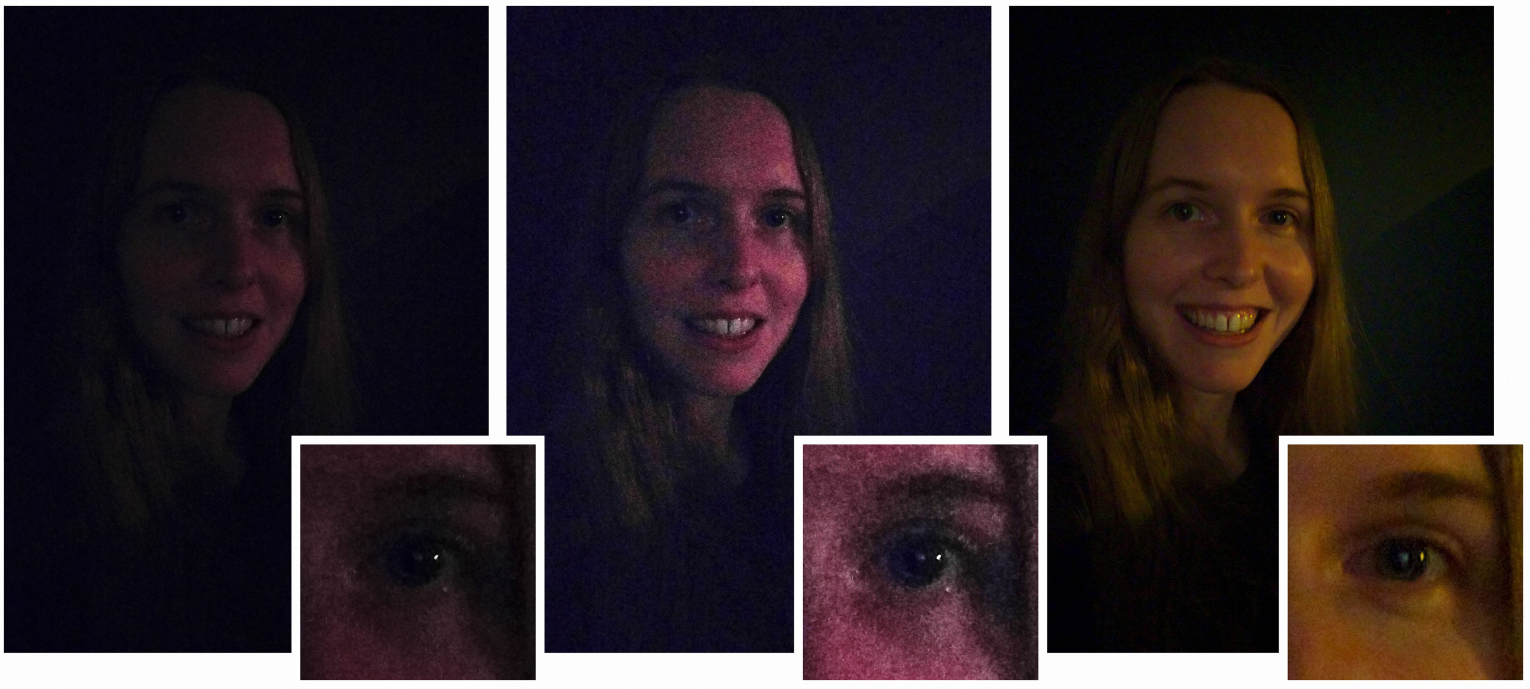
\includegraphics[width=0.95\linewidth]{imgs/burstgoogle}
 \caption{Comparação dos pipelines de fotografia: A esquerda temos uma imagem usando o pipeline tradicional; a do meio usando aumento de contraste e remoção de ruido; e a da direita mostra o novo pipeline desenvolvido pelos autores.} 
 \label{fig:burstgoogle} 
\end{figure}

O artigo é contextualizado no tratamento de imagens de cameras de smartphones. A característica a ser abordada é  a limitação que quantidade de elétrons que cada sensor da matriz de sensitiva pode armazenar. Esse problema se evidencia em imagens com baixa luminosidade. Os autores desenharam um pipeline que captura, alinha e une um conjunto de frames tomados com exposição constante. O resultado é ter sombras bem delineadas e \textit{profundidade de contraste} maior, o que permite a aplicação de algoritmos de HDR e Tone Mapping. 

Para alcançar o resultados a imagem processada foi em formato RAW e não a demosaiçada (bayer filters) proveniente dos do hardware de processamento de sinais de imagem (ISP). Ao utilizar imagens em formato RAW, o dado chega com maior quantidade de bits por pixel, alem de evitar a execução indesejada de HDR, Tone Mapping e remoção de ruído do ISP.

Em cima disso, desenvolveram uma abordagem de alinhamento baseado em FFT e um hibrido 2D/3D do filtro Weiner para remoção de ruídos.

Na minha opinião, o que faz este artigo relevante para o que foi explicado inicialmente na disciplina é a abordagem de pegar os dados em formato RAW antes de passar pelo processamento do ISP. Isto permite tratar o dado com informações mais ricas, podendo aumentar a profundidade de bits de cada pixel. Ao usar frames com a mesma abertura e tempo de exposição, facilita o funcionamento do algoritmo de alinhamento. Deixar a camera com exposição maior leva a efeitos indesejados como o ghosting.

\textbf{4) Fazer resumo da próxima aula:}
\begin{itemize}
\item Livro : GONZALEZ, RAFAEL C. e WOODS, RICHARD E.; Digital image processing. Massachusets: Addison-Wesley, 1993. 716p. \cite{Gonzalez02a}
\item Fazer resumo dos capítulos 2 e 4: máximo uma página para cada capítulo (ver instruções na aula 1)
\item Procurar os assuntos abordados em outros livros de Processamento de Imagens. Citar bibliografia utilizada no final (não conta na página do resumo).
\item Construir pelo menos 2 questões para discussão de cada capítulo.
\end{itemize}

\pagebreak

\textbf{Capítulo 2:} Fundamentos da imagem digital

Este capítulo é focado em apresentar os fundamentos necessários para o entendimento dos conceitos de imagem digital. É dividido em 5 seções:

\textit{2.1 Elementos da Percepção visual} Aborda como a imagem é formada no olho humano. 

O olho humano possui diversas estruturas, mas para a simplicidade de explicação descreverei brevemente alguns deles:

\begin{description}
\item{Córnea} é a estrutura mais externa e transparente que separa o olho do meio ambiente;
\item{Íris} é a estrutura que controla a quantidade de luz que entra dentro do olho;
\item{Cristalino} é uma lente que pode mudar o foco devido a contração de músculos para melhor adequar o posicionamento da formação da imagem no olho.
\item{Retina} é onde a imagem é formada e contém os neurônios sensíveis a luz, os cones e os bastonetes. 
\end{description}

\textit{2.2 A luz e o espectro eletromagnético} usa uma abordagem mais matemática e física sobre como a luz se comporta e quais os impactos na formação da imagem.

A equação $\lambda=\frac{c}{\nu}$ descreve a relação do comprimento de onda $\lambda$ com a velocidade da luz $c$ e a frequência da onda $\nu$. O que mostra que quanto maior for o comprimento de onda, menor é sua frequência.

A equação $E=h\nu$ descreve como a energia do foton $E$ se relaciona com a frequência da onda $\nu$ através da constante universal de Plank $h$.

\textit{2.3 Sensores e aquisição de imagens} aborda como sensores são feitos, construidos e combinados de tal forma a captar imagens; 

A aquisição de imagem pode ser feita de diversas maneiras como um sensor único que varre a área de interesse como nos microscópios eletrônicos de varredura, ou então utilizam matriz de sensores.

Em ambos os casos o sensor é um poço de potencial que acumula estímulos por determinado tempo. Inicialmente ele é configurado para um valor inicial e a medida que o estímulo chega (por exemplo fótons que liberam elétrons), o poço aprisiona a informação (acumula diferença de potencial) para medir o valor do que foi acumulado durante o intervalo de tempo. 

\textit{2.4 Amostragem e quantização de imagens} aborda métodos utilizados para amostrar informação do sinal luminoso e valorar a sua intensidade; 

Os sensores acumulam valores contínuos de informação e além disso o poço de potencial possui limiar do que consegue conter. Tendo isto em mente, para armazenar a informação na forma de bits, é preciso quantizar quais faixas de valores contínuos se equiparam com qual valor discreto.  

\textit{2.5 Alguns relacionamentos básicos entre pixels} aborda conceitos de relacionamentos entre pixels.

Ao analisar pixels de uma imagem, precisa-se descrever conceitos de vizinhança, distância e adjacências. 

\textit{2.6 Uma introdução às ferramentas matemáticas utilizadas no processamento digital de imagens} discute operadores aritméticos, lógicos, matriciais.

Operadores que são aplicados a imagem de maneira geral modificam a imagem com alguma intenção específica. Por exemplo operadores de adição com uma máscara móvel é bastante útil para se fazer um filtro de média para suavizar a imagem. Já transformadas afins como rotação, escala e cisalhamento são importantes para modificar o mapeamento da localização das informações na imagem.

A transformada de Fourier é muito importante e será discutida mais a fundo no capitulo 4.

\pagebreak
\twocolumn
\textbf{Capítulo 4: } Filtragem no domínio da frequência.

Este capítulo aborda as bases para o entendimento da transformada de Fourier; os princípios básicos da amostragem de funções; as transformadas discretas de Fourier uni e bidimensionais; a amostragem por aliasing; filtragem no domínio da
frequência: técnicas de filtragem para aguçamento e suavização.

\textbf{4.1 Fundamentos}

Esta seção aborda um breve histórico da série e da transformada de Fourier e o porquê dela ser tão importante e influenciar várias áreas da matemática. 

Seu estudo inicialmente se focou em analisar o calor. Apesar de ondas de calor serem estáveis, até funções não periódicas podem ser expressas como uma integral de senos e/ou cossenos multiplicada por uma função de ponderação. A formulação nesse caso é a transformada de Fourier.

\textbf{4.2 Conceitos Preliminares}

Nesta seção, o autor aborda definições básicas que serão usadas para descrever a série de Fourier.

\textbf{4.3 Amostragem e a transformada de Fourier de funções amostradas}

São descritas as bases para expressar matematicamente a amostragem. O que leva aos princípios básicos da transformada de Fourier de amostras de funções. 

Um conceito importante descrito é o de Aliasing: é quando uma função de banda limitada é amostrada em uma taxa menor que o dobro de sua frequência mais alta. O efeito final da redução da taxa de amostragem abaixo da taxa de Nyquist é que os períodos agora se sobrepõem, e passa a ser impossível isolar um único período da transformada.

\textbf{4.4 A transformada discreta de Fourier (DFT) de uma variável}
Esta seção foca em deduzir a transformada discreta de Fourier (DFT, de discrete Fourier transform).

\textbf{4.5 Extensão para funções de duas variáveis}

Mostra como estender o conceito da transformada 1D para 2D. Aborda Aliasing em imagens, interpo- lação e reamostragem.

\textbf{4.6 Algumas propriedades da transformada discreta de Fourier 2-D}

Relacionamentos entre intervalos no espaço e na frequência; Translação e rotação; Periodicidade; Simetria; Ângulo de fase; Convolução 2D;

\textbf{4.7 Os fundamentos da filtragem no domínio da frequência}

Características e fundamentos da filtragem no domínio da frequência;

\textbf{4.8 Suavização de imagens utilizando filtros no domínio da frequência}

Filtro passa-baixa ideal deixa passar, todas as frequências em um círculo de raio R a partir da origem e recorta todas as frequências fora desse círculo. Já filtro passa-baixa Butterworth não tem uma descontinuidade abrupta que resulta em um corte bem definido entre frequências passadas e filtradas. Os filtros passa-baixa gaussianos são ligeiramente menos suaves. No caso de imagens médicas, o Butterworth é preferível pois controla melhor as transições entre alta e baixa frequencia.

\textbf{4.9 Aguçamento de imagens utilizando filtros no domínio da frequência}

É teóricamente o oposto do filtro passa-baixa. Elimina todas as frequências dentro de um círculo de raio R enquanto passa, todas as frequências fora do círculo. Como as propriedades são similares, também ocorre o fenômeno de ringing. Esses filtros podem ser usados como realce de imagem por valorizar divergências entre vizinhos. 

\textbf{4.10 Filtragem seletiva}

Filtros rejeita-banda e passa-banda. São construidos usando os conceitos de passa-alta e passa-baixa. Um caso específico disso é o filtro notch, cuja a principal finalidade é remover padrão moiré de imagens antigas de impressão de revistas e jornais quando digitalizados.

\textbf{4.11 Implementação}

Nesta parte, o autor foca em ensinar como implementar e desenhar filtros que usem transformada de fourier e uma implementação bastante comum: FFT, a transformada rápida de fourier.

\pagebreak
\onecolumn
\textbf{Perguntas:}

\textbf{Cap. 2:} Por que os filtros bayesianos de cor nos sensores de câmeras possuem mais sensores de cor verde do que os demais? Qual a vantagem das TVs usarem o padrão RGBW para representar as cores? \cite{li2015design}

\textbf{Cap. 4:} O que é o Nyquist frequency? \cite{tang2016design}

\bibliographystyle{sbgames}
\bibliography{template}
\end{document}